\documentclass[12pt,a4paper,notitlepage]{article}
% dans ce modèle article ne pas utiliser la mention "chapter", par contre on peut
% utiliser la numérotation naturelle et les références croisées.
\usepackage[utf8x]{inputenc}
\usepackage{ucs}
\usepackage[french]{babel}
\usepackage[T1]{fontenc}
%\usepackage{eurosym} % pour pouvoir utiliser le symbole \euro{}
\usepackage[left=17mm,right=17mm,top=17mm,bottom=17mm]{geometry}
% définition du nombre de lignes à afficher en fin ou en début de page pour
% éviter les veuves et orphelines.
\usepackage[all, defaultlines=3]{nowidow}
\usepackage{array}
\usepackage[table]{xcolor} % pour couleur de blocs, permis avec \color{couleur}{texte}

\usepackage{multirow}
\usepackage{multicol}
	\setlength{\columnsep}{0.6cm}
	\setlength{\columnseprule}{1pt}
	\def\columnseprulecolor{\color{black}}

%\usepackage{wrapfig}
% \begin{wrapfigure}[lineheight]{position = r R l L i I o O}{width}
%  minuscule = float, majuscule = force emplacement
% \end{wrapfigure}

\usepackage{hyperref} %support des url via le tag \url
\hypersetup{
	colorlinks=true,
	linkcolor=blue,
	urlcolor=purple,
	}
	\urlstyle{same}
\usepackage{amsmath}
\usepackage{amsfonts}
\usepackage{amssymb}
	\everymath{\displaystyle}
%\usepackage{textcomp}

\usepackage{graphicx}
%\graphicspath{ {./Images/} } % indique le chemin relatif où sont situées les images
% définition de la clé Graphic Inclusion pour paramétrer par défaut la taille des images incluses
	\setkeys{Gin}{width=0.500\linewidth}
\usepackage{float}
	\floatplacement{table}{H} %par défaut tables là où code est posé
	\floatplacement{figure}{H} %par défaut images là où code est posé
%\usepackage{siunitx}
%	\sisetup{locale = FR}
%%%% Packet circuitikz permet de dessiner des circuits électriques, peut nécessiter l'utiliation de siunitx
%\usepackage[european]{circuitikz}
%\usetikzlibrary{babel}
%\usepackage{qrcode}
%\usepackage{pgfplots} %permet de tracer directement des graphiques depuis latex

\usepackage{ifthen}
%%% Gestion de la dyslexie
\newboolean{isDyslexique}
	\setboolean{isDyslexique}{false}
%%% Gestion de la correction
\newboolean{isCorrection}
	\setboolean{isCorrection}{false}

% \usepackage{palatino} %\usepackage{sans}
% \usepackage{lxfonts} %\usepackage{arev}
\ifthenelse{\boolean{isDyslexique}}{% si vrai :
	\usepackage{arev}
	\renewcommand{\baselinestretch}{1.5}
}{% si faux :
	\usepackage{lmodern}
%	\usepackage{sans}
	\renewcommand{\baselinestretch}{1.25}
}
\usepackage{lastpage}
% test de modification des headers et footers
\usepackage{fancyhdr}
\pagestyle{fancy}
\fancyhf{}
\fancyhead[LE,RO]{\rightmark}
\fancyhead[LO,RE]{\leftmark}
\fancyfoot[LE,RO]{F.S.G.}
\fancyfoot[C]{.::--- \ \thepage / \pageref*{LastPage} \ ---::.}
\fancyfoot[RE,LO]{c4-1·pd·ac2}
% fin du test de modification :)
\usepackage{tikz}
	\usetikzlibrary{babel,math}
% inclusion du paquet bclogo pour boîtes avec logo de mise en exergue
\usepackage[tikz]{bclogo}

% ========= DÉFINITION D'UN INTERLIGNE DIFFÉRENT ===============
\setlength{\parskip}{0.1cm} % définit l'espacement entre paragraphes
\renewcommand{\thesection}{\Roman{section}}

\author{F.G.}
% éviter le titre peut-être ?
\title{}

\begin{document}

\begin{flushleft}
\begin{tabular}{| m{0.15\linewidth}  m{0.8\linewidth} || }
	\hline
	\multirow{4}{*}{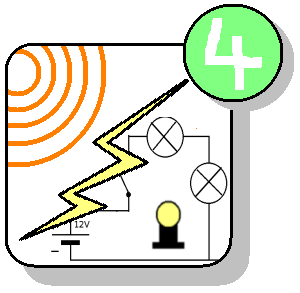
\includegraphics[width=\linewidth]{cycle4-logo-elec-ondes-nrj.png}} 
	& c4-1·pd·ac2
	\begin{LARGE}
		La lumière transporte la couleur.
	\end{LARGE} \cr
	\cline{2-2}
	 & \cr
	 & Nom : . \ \ . \ \ . \ \ . \ \ . \ \ . \ \ . \ \ . Prénom : . \ \ . \ \ . \ \ . \ \ . \ \ . \cr
	 & \cr
	 & Groupe : . \ \ . \ \ . \ \ . Durée : 50 min. \cr
	\hline\hline
\end{tabular}
\end{flushleft}

% ======== LISTE DES IMAGES DISPONIBLES POUR CYCLES 3 ET 4 =========
% 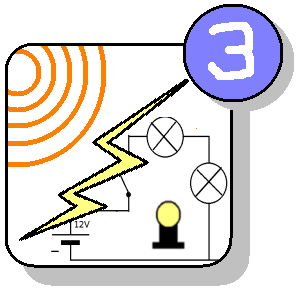
\includegraphics[scale=0.333]{cycle3-logo-elec-ondes-nrj.png}
% 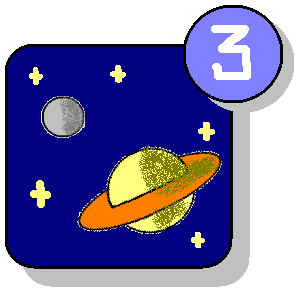
\includegraphics[scale=0.333]{cycle3-logo-espace.png}
% 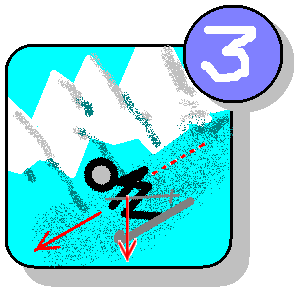
\includegraphics[scale=0.333]{cycle3-logo-mvts.png}
% 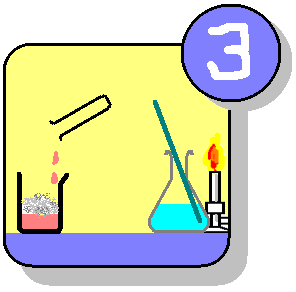
\includegraphics[scale=0.333]{cycle3-logo-transfo-matiere.png}
% 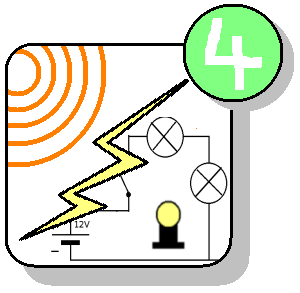
\includegraphics[scale=0.333]{cycle4-logo-elec-ondes-nrj.png}
% 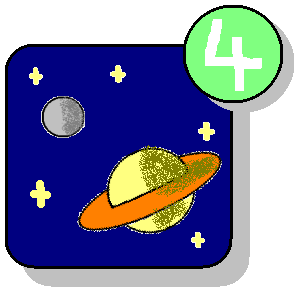
\includegraphics[scale=0.333]{cycle4-logo-espace.png}
% 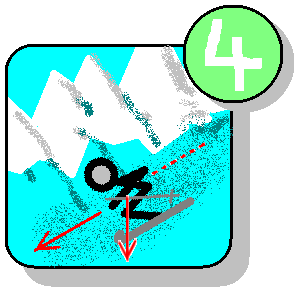
\includegraphics[scale=0.333]{cycle4-logo-mvts.png}
% 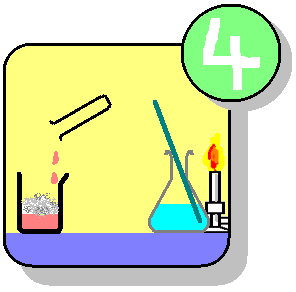
\includegraphics[scale=0.333]{cycle4-logo-transfo-matiere.png}

%\begin{flushleft}
%\begin{tabular}{| m{0.15\linewidth} | m{0.8\linewidth} ||}
%	\hline
%	NOTE : & APPRÉCIATION : \cr
%	$ ~~ $ & $ ~~ $ \cr
%	$ ~~ $ & $ ~~ $ \cr
%	$ ~~ $ & $ ~~ $ \cr
%	$ ~~ $ & $ ~~ $ \cr
%	$ ~~ $ & $ ~~ $ \cr
%	\hline\hline
%\end{tabular}
%\end{flushleft}

% $ ~~ $

\begin{flushleft}
\begin{tabular}{| m{0.03\linewidth} | m{0.75\linewidth} || m{0.015\linewidth} | m{0.015\linewidth} | m{0.015\linewidth} | m{0.015\linewidth} || }
\hline
\multirow{2}{*}{Ref} & \multirow{2}{*}{i~n~t~i~t~u~l~é~~~ d~e~~~ l~a~~~ c~o~m~p~é~t~e~n~c~e (cycle4) } & \multicolumn{4}{c ||}{É~t~a~t} \cr
	\cline{3-6}
	& & I & F & S & T \cr \hline
% A & Pratiquer des démarches scientifiques \cr \hline
%	A1 & \footnotesize{Identifier des questions de nature scientifique.} & & & & \cr \hline
%	A2 & \footnotesize{Proposer une ou des hypothèses pour répondre à une question scientifique. \newline Concevoir une expérience pour la ou les tester.} & & & & \cr \hline
	A3 & \footnotesize{Mesurer des grandeurs physiques de manière directe ou indirecte.} & & & & \cr \hline
%	A4 & \footnotesize{Interpréter des résultats expérimentaux, en tirer des conclusions et les communiquer en argumentant.} & & & & \cr \hline
%	A5 & \footnotesize{Développer des modèles simples pour expliquer des faits d'observations et mettre en \oe{}uvre des démarches propres aux sciences.} & & & & \cr \hline
% B & Concevoir, créer, réaliser \cr \hline
%	B1 & \footnotesize{Concevoir et réaliser un dispositif de mesure ou d'observation.} & & & & \cr \hline
% C & S'approprier des outils et des méthodes \cr \hline
%	C1 & \footnotesize{Effectuer des recherches bibliographiques.} & & & & \cr \hline
%	C2 & \footnotesize{Utiliser des outils numériques pour mutualiser des informations sur un sujet scientifique.} & & & & \cr \hline
%	C3 & \footnotesize{Planifier une tâche expérimentale, organiser son espace de travail, garder des traces des étapes suivies et des résultats obtenus.} & & & & \cr \hline
% D & Pratiquer des langages \cr \hline
%	D1 & \footnotesize{Lire et comprendre des documents scientifiques.} & & & & \cr \hline
%	D2 & \footnotesize{Utiliser la langue française en cultivant précision, richesse de vocabulaire et syntaxe pour rendre compte des observations, expériences, hypothèses et conclusions.} & & & & \cr \hline
%	D3 & \footnotesize{S'exprimer à l'oral lors d'un débat scientifique.} & & & & \cr \hline
	D4 & \footnotesize{Passer d'une forme de langage scientifique à une autre.} & & & & \cr \hline
% E & Mobiliser des outils numériques \cr \hline
	E1 & \footnotesize{Utiliser des outils d'acquisition et de traitement de données, de simulations et de modèles numériques.} & & & & \cr \hline
%	E2 & \scriptsize{Produire des documents scientifiques grâce à des outils numériques, en utilisant l'argumentation et le vocabulaire spécifique à la physique et à la chimie.} & & & & \cr \hline
% F & Adopter un comportement éthique et responsable \cr \hline
%	F1 & \scriptsize{Expliquer les fondements des règles de sécurité en chimie, électricité et acoustique. Réinvestir ces connaissances ainsi que celles sur les ressources et sur l'énergie, pour agir de façon responsable.} & & & & \cr	\hline
%	F2 & \footnotesize{S'impliquer dans un projet ayant une dimension citoyenne.} & & & & \cr	\hline
% G & Se situer dans l'espace et dans le temps \cr \hline
%	G1 & \footnotesize{Expliquer, par l'histoire des sciences et des techniques, comment les sciences évoluent et influencent la société.} & & & & \cr	\hline
%	G2 & \footnotesize{Identifier les différentes échelles de structuration de l'Univers.} & & & & \cr \hline
	\hline
\end{tabular}
\end{flushleft}
% ============= DÉBUT DU DOCUMENT DE TRAVAIL ==================

\paragraph*{Point du programme abordé / Objectif.} \og~Signal et information.~\fg{}
\og~\emph{Comprendre que l'utilisation du son et {\bf de la lumière}} permet d'émettre, de transporter un signal donc une information\/~\fg{}.

\paragraph*{Matériel à disposition.}
Chaque table dispose~:
\begin{itemize}
	\item une tablette ;
%	\item un objectif de microscope.
\end{itemize}

\section*{Question :} Comment sur un écran (smartphone, télé, ordinateur ...) ou avec des projecteurs, peut-on créer la grande majorité des couleurs que peut voir un \oe{}uil humain ? 

En effectuant les différentes tâches qui suivent, comprenez comment on peut \og~coder~\fg{} des couleurs puis répondez à la question.

\section{Expérimentation.}

Chaque groupe dispose du matériel posé sur sa paillasse. 
Laissez-vous guider par les différentes tâches.

\subsection*{Exemples.}
\paragraph*{doc1. Exemple d'affiche.}
Observation d'une affiche amenée en classe avec un smartphone + objectif de microscope pour pouvoir prendre en photo un zoom très rapproché d'un point de l'affiche.

\paragraph*{doc2.} Zoom sur une capture d'écran.
\begin{figure}
	\centering
	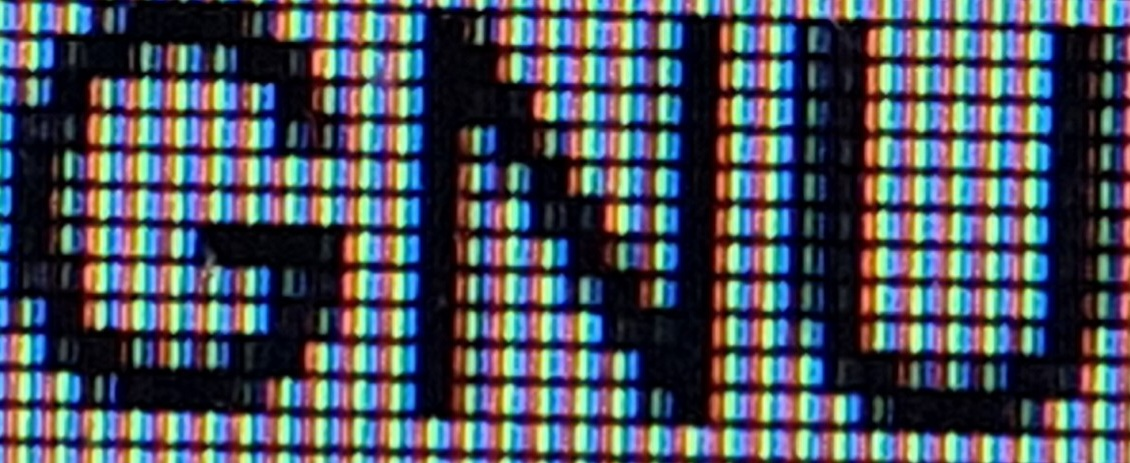
\includegraphics{gnu.jpg}
\end{figure}

\subsection*{tâche 1 : appropriation de l'application.}
Sur la tablette ouvre l'application \texttt{RVB Tool} voici sa très brève description :

\paragraph{Zone haute.}
Cette zone contient trois lignes~:
\begin{itemize}
	\item une ligne ``RVB'' où figurent les trois couleurs Rouge, Vert et Bleu ainsi que l'opacité. Chacun des 4 paramètres va de 0 à 255.
	\item une ligne ``TSL'' qui ne sera pas utilisée pendant cette activité.
	\item une ligne ``HEX'' où est transformée l'opacité, le rouge, le vert et le bleu non pas de 0 à 255 mais de 00 à FF.
\end{itemize}
\begin{figure}
	\centering
	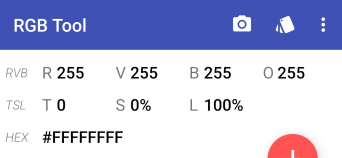
\includegraphics{zone-haute.png}
\end{figure}

\paragraph{Zone centrale.}
La zone centrale affiche la couleur réglée grâce à la zone basse et dont les réglages sont affichés en zone haute.

\paragraph{Zone basse.}
La zone basse contient 4 curseurs (ronds), réglant l'Opacité (O), le rouge (R), le bleu (B) et le vert (V).
\begin{figure}
	\centering
	
\includegraphics{zone-basse.png}
\end{figure}

\begin{bclogo}[logo=\bccrayon, couleur=yellow!5, arrondi=0.1, nobreak]{Activité :}
Réglez les différents curseurs dans la zone basse afin de découvrir tout ce qui change dans les informations affichées et pour faire connaissance avec l'application.
La durée maximale de cette prise en main est 5 minutes.
\end{bclogo}

\subsection*{tâche 2 : Expérimentation et collecte des résultats.}
En utilisant les curseurs réglez les couleurs aux valeurs indiquées dans le tableau et complétez toutes les lignes.
\begin{table}
	\centering
	\renewcommand*{\arraystretch}{1.25}
	\begin{tabular}{| m{0.35\linewidth} | m{0.05\linewidth} | m{0.05\linewidth} | m{0.05\linewidth} | m{0.05\linewidth} | m{0.15\linewidth} |}
		\hline
		Couleur observée & O & R & V & B & Hexadécimal \cr
		\hline
		& 255 & 0 & 0 & 255 & \cr
		\hline
		& 255 & 0 & 255 & 0 & \cr
		\hline
		& 255 & 255 & 0 & 0 & \cr
		\hline
		& 255 & 255 & 255 & 0 & \cr
		\hline
		& 255 & 255 & 0 & 255 & \cr
		\hline
		& 255 & 0 & 255 & 255 & \cr
		\hline
		& 255 & 0 & 0 & 0 & \cr
		\hline
		& 255 & 255 & 255 & 255 & \cr
		\hline
		& 255 & 255 & 192 & 64 & \cr
		\hline
		& 255 & 150 & 98 & 23 & \cr
		\hline
		& & & & & \#{}FF 7C 21 C1 \cr
		\hline
		& 0 & 255 & 255 & 255 & \cr
		\hline
	\end{tabular}
\end{table}

\subsection*{tâche 3 : Analyse des résultats}
\begin{bclogo}[couleur=yellow!5, arrondi=0.1, logo=\bccrayon, nobreak=true]{}
	Répondez aux questions avant d'effectuer la tâche suivante.
\end{bclogo}
\paragraph{1.} Quelles sont les couleurs utilisées dans le logiciel ? \newline
\noindent . \ \ . \ \ . \ \ . \ \ . \ \ . \ \ . \ \ . \ \ . \ \ . \ \ . \ \ . \ \ .
\ \ . \ \ . \ \ . \ \ . \ \ . \ \ . \ \ . \ \ . \ \ . \ \ . \ \ . \ \ . \ \ . \ \ . 
\ \ . \ \ . \ \ . \ \ . \ \ . \ \ . \ \ . \ \ . \ \ . \ \ . \ \ . \ \ . \ \ . \ \ . 
\ \ . \ \ . \ \ . \ \ . \ \ . \ \ . \ \ . \ \ . \ \ . \ \ . \ \ . \ \ . \ \ . \ \ . 
\ \ . \ \ . \ \ . \ \ . \ \ . \ \ . \ \ . \ \ . \ \ . \ \ . \ \ . \ \ . \ \ . \ \ . 
\ \ . \ \ . \ \ . \ \ . \ \ . \ \ . \ \ . \ \ . \ \ . \ \ . \ \ . \ \ . \ \ . \ \ . 

\paragraph{2.} Avez-vous réussi à former des couleurs différentes grâce aux trois couleurs de la question précédente ?
\noindent . \ \ . \ \ . \ \ . \ \ . \ \ . \ \ . \ \ . \ \ . \ \ . \ \ . \ \ . \ \ .
\ \ . \ \ . \ \ . \ \ . \ \ . \ \ . \ \ . \ \ . \ \ . \ \ . \ \ . \ \ . \ \ . \ \ . 
\ \ . \ \ . \ \ . \ \ . \ \ . \ \ . \ \ . \ \ . \ \ . \ \ . \ \ . \ \ . \ \ . \ \ . 
\ \ . \ \ . \ \ . \ \ . \ \ . \ \ . \ \ . \ \ . \ \ . \ \ . \ \ . \ \ . \ \ . \ \ . 
\ \ . \ \ . \ \ . \ \ . \ \ . \ \ . \ \ . \ \ . \ \ . \ \ . \ \ . \ \ . \ \ . \ \ . 
\ \ . \ \ . \ \ . \ \ . \ \ . \ \ . \ \ . \ \ . \ \ . \ \ . \ \ . \ \ . \ \ . \ \ . 

\paragraph{3.} Quel est le résultat de $2 \times 2 \times 2 \times 2 \times 2 \times 2 \times 2 \times 2$ ? Si on commence à compter depuis zéro, quelle est le nombre maximal qui puisse être obtenu ?
\noindent . \ \ . \ \ . \ \ . \ \ . \ \ . \ \ . \ \ . \ \ . \ \ . \ \ . \ \ . \ \ .
\ \ . \ \ . \ \ . \ \ . \ \ . \ \ . \ \ . \ \ . \ \ . \ \ . \ \ . \ \ . \ \ . \ \ . 
\ \ . \ \ . \ \ . \ \ . \ \ . \ \ . \ \ . \ \ . \ \ . \ \ . \ \ . \ \ . \ \ . \ \ . 
\ \ . \ \ . \ \ . \ \ . \ \ . \ \ . \ \ . \ \ . \ \ . \ \ . \ \ . \ \ . \ \ . \ \ . 
\ \ . \ \ . \ \ . \ \ . \ \ . \ \ . \ \ . \ \ . \ \ . \ \ . \ \ . \ \ . \ \ . \ \ . 
\ \ . \ \ . \ \ . \ \ . \ \ . \ \ . \ \ . \ \ . \ \ . \ \ . \ \ . \ \ . \ \ . \ \ . 

\subsection*{tâche 4 : Réponse à la question}
Dans le cadre qui suit, répondez à la question posée au début.
\begin{bclogo}[couleur=yellow!5, arrondi=0.1, logo=\bccrayon, nobreak=true]{}

\noindent . \ \ . \ \ . \ \ . \ \ . \ \ . \ \ . \ \ . \ \ . \ \ . \ \ . \ \ . \ \ .
\ \ . \ \ . \ \ . \ \ . \ \ . \ \ . \ \ . \ \ . \ \ . \ \ . \ \ . \ \ . \ \ . \ \ . 
\ \ . \ \ . \ \ . \ \ . \ \ . \ \ . \ \ . \ \ . \ \ . \ \ . \ \ . \ \ . \ \ . \ \ . 
\ \ . \ \ . \ \ . \ \ . \ \ . \ \ . \ \ . \ \ . \ \ . \ \ . \ \ . \ \ . \ \ . \ \ . 
\ \ . \ \ . \ \ . \ \ . \ \ . \ \ . \ \ . \ \ . \ \ . \ \ . \ \ . \ \ . \ \ . \ \ . 
\ \ . \ \ . \ \ . \ \ . \ \ . \ \ . \ \ . \ \ . \ \ . \ \ . \ \ . \ \ . \ \ . \ \ . 
\ \ . \ \ . \ \ . \ \ . \ \ . \ \ . \ \ . \ \ . \ \ . \ \ . \ \ . \ \ . \ \ . \ \ . 
\ \ . \ \ . \ \ . \ \ . \ \ . \ \ . \ \ . \ \ . \ \ . \ \ . \ \ . \ \ . \ \ . \ \ . 
\ \ . \ \ . \ \ . \ \ . \ \ . \ \ . \ \ . \ \ . \ \ . \ \ . \ \ . \ \ . \ \ . \ \ . 
\ \ . \ \ . \ \ . \ \ . \ \ . \ \ . \ \ . \ \ . \ \ . \ \ . \ \ . \ \ . \ \ . \ \ . 
\ \ . \ \ . \ \ . \ \ . \ \ . \ \ . \ \ . \ \ . \ \ . \ \ . \ \ . \ \ . \ \ . \ \ . 

\end{bclogo}

\section{À retenir.}
\begin{bclogo}[couleur=pink!5, arrondi=0.1, logo=\bccoeur, nobreak=true]{}
\ifthenelse{\boolean{isCorrection}}{% is true
{\Large
	{\color{red}
	La lumière permet de transformer de l'information sous forme de couleur.
	
	Certaines couleurs sont dites \og~primaires~\fg{}~: il s'agit du rouge, du vert et eu bleu.
	
	En additionnant les couleurs primaires avec différentes intensités lumineuses on peut former la grande majorité des couleurs que l'\oe{}il humain capte.
	} % end red	

	Le codage informatique traditionnel (1 octet pour le rouge, 1 pour le vert et 1 pour le bleu) permet d'obtenir des intensités allant de 0 à 255 (décimal) ou de 00 à FF (hexadécimal) ce qui permet de coder 16~777~216 couleurs.
	
	Un code d'opacité permet aussi d'ajouter de la transparence.
} % end large
}{% else
\noindent . \ \ . \ \ . \ \ . \ \ . \ \ . \ \ . \ \ . \ \ . \ \ . \ \ . \ \ . \ \ .
\ \ . \ \ . \ \ . \ \ . \ \ . \ \ . \ \ . \ \ . \ \ . \ \ . \ \ . \ \ . \ \ . \ \ . 
\ \ . \ \ . \ \ . \ \ . \ \ . \ \ . \ \ . \ \ . \ \ . \ \ . \ \ . \ \ . \ \ . \ \ . 
\ \ . \ \ . \ \ . \ \ . \ \ . \ \ . \ \ . \ \ . \ \ . \ \ . \ \ . \ \ . \ \ . \ \ . 
\ \ . \ \ . \ \ . \ \ . \ \ . \ \ . \ \ . \ \ . \ \ . \ \ . \ \ . \ \ . \ \ . \ \ . 
\ \ . \ \ . \ \ . \ \ . \ \ . \ \ . \ \ . \ \ . \ \ . \ \ . \ \ . \ \ . \ \ . \ \ . 
\ \ . \ \ . \ \ . \ \ . \ \ . \ \ . \ \ . \ \ . \ \ . \ \ . \ \ . \ \ . \ \ . \ \ . 
\ \ . \ \ . \ \ . \ \ . \ \ . \ \ . \ \ . \ \ . \ \ . \ \ . \ \ . \ \ . \ \ . \ \ . 
\ \ . \ \ . \ \ . \ \ . \ \ . \ \ . \ \ . \ \ . \ \ . \ \ . \ \ . \ \ . \ \ . \ \ . 
\ \ . \ \ . \ \ . \ \ . \ \ . \ \ . \ \ . \ \ . \ \ . \ \ . \ \ . \ \ . \ \ . \ \ . 
\ \ . \ \ . \ \ . \ \ . \ \ . \ \ . \ \ . \ \ . \ \ . \ \ . \ \ . \ \ . \ \ . \ \ . 
\ \ . \ \ . \ \ . \ \ . \ \ . \ \ . \ \ . \ \ . \ \ . \ \ . \ \ . \ \ . \ \ . \ \ . 
\ \ . \ \ . \ \ . \ \ . \ \ . \ \ . \ \ . \ \ . \ \ . \ \ . \ \ . \ \ . \ \ . \ \ . 
\ \ . \ \ . \ \ . \ \ . \ \ . \ \ . \ \ . \ \ . \ \ . \ \ . \ \ . \ \ . \ \ . \ \ . 
\ \ . \ \ . \ \ . \ \ . \ \ . \ \ . \ \ . \ \ . \ \ . \ \ . \ \ . \ \ . \ \ . \ \ . 
\ \ . \ \ . \ \ . \ \ . \ \ . \ \ . \ \ . \ \ . \ \ . \ \ . \ \ . \ \ . \ \ . \ \ . 
\ \ . \ \ . \ \ . \ \ . \ \ . \ \ . \ \ . \ \ . \ \ . \ \ . \ \ . \ \ . \ \ . \ \ . 
} %end of else
\end{bclogo}

\section{Apparté.}
\paragraph{note :} Cet apparaté est plutôt réservé aux classes dont les résultats sont excellents globalement. Consigne : compléter les zones de croisement des cercles avec les couleurs appropriées
\begin{figure}
	\centering
	\begin{tikzpicture}
%		\draw[dashed, blue, thin, step=0.5cm] (-3,-2.5) grid (5,4) ;
		\foreach \x/\y in {0/0, 3/0, 1.5/2.5}{%
			\draw (\x,\y) circle (2) ;
		} ;
		\ifthenelse{\boolean{isCorrection}}{%
			\draw[<-, purple] (2,3) -- ++(3,0) node[right]{Rouge} ;
			\draw[<-, purple] (2.6,1.6) -- ++(3,0) node[right]{Jaune} ;
			\draw[<-, purple] (4,-0.5) -- ++(3,0) node[right]{Vert} ;
			\draw[<-, purple] (1.5,0.9) -- ++(5,-0.5) node[right]{Blanc} ;
			\draw[<-, purple] (-1,-1) -- ++(-3,0) node[left]{Bleu} ;
			\draw[<-, purple] (0.6,1.1) -- ++(-3,0) node[left]{Magenta} ;
			\draw[<-, purple] (1.6,0) -- ++(-5,0) node[left]{Cyan} ;	
		}{%
			\draw[<-, purple] (2,3) -- ++(3,0) node[right]{Rouge} ;
			\draw[<-, purple] (2.6,1.6) -- ++(3,0) node[right]{} ;
			\draw[<-, purple] (4,-0.5) -- ++(3,0) node[right]{Vert} ;
			\draw[<-, purple] (1.5,0.9) -- ++(5,-0.5) node[right]{} ;
			\draw[<-, purple] (-1,-1) -- ++(-3,0) node[left]{Bleu} ;
			\draw[<-, purple] (0.6,1.1) -- ++(-3,0) node[left]{} ;
			\draw[<-, purple] (1.6,0) -- ++(-5,0) node[left]{} ;	
		}
	\end{tikzpicture}
\end{figure}
\ifthenelse{\boolean{isCorrection}}{%if true
	Ceci est le diagramme de la synthèse additive des couleurs, l'addition de deux couleurs primaires (R, V, B) donne une couleur secondaire (Jaune, Cyan, Magenta), l'addition des trois donne du blanc.
}{%if false
\noindent . \ \ . \ \ . \ \ . \ \ . \ \ . \ \ . \ \ . \ \ . \ \ . \ \ . \ \ . \ \ .
\ \ . \ \ . \ \ . \ \ . \ \ . \ \ . \ \ . \ \ . \ \ . \ \ . \ \ . \ \ . \ \ . \ \ . 
\ \ . \ \ . \ \ . \ \ . \ \ . \ \ . \ \ . \ \ . \ \ . \ \ . \ \ . \ \ . \ \ . \ \ . 
}

\end{document}

%%%%%%%%%%%%%%%%%%%%%%%%%%%%%%%%%%%%%%%%%%%%%%%%%%%%%%%

% cadre pour le cours / à savoir par coeur.
\begin{bclogo}[couleur=pink!5, epOmbre=0.2cm, arrondi=0.1, logo=\bccoeur, nobreak=true]{}

\end{bclogo}

% cadre pour un document à analyser (informatif)
\begin{bclogo}[couleur=blue!5, epOmbre=0.2cm, arrondi=0.1, logo=\bcinfo, nobreak=true]{}

\end{bclogo}

% cadre pour le travail :
\begin{bclogo}[couleur=yellow!5, arrondi=0.1, logo=\bccrayon, nobreak=true]{}

\end{bclogo}